\section{Introduction}

X-ray absorption and Auger electron spectroscopies are powerful tools to study the electronic structure and the nearest environment of atoms and molecules in gas, liquid and solid phase. Understanding how atoms or molecules respond to irradiation with x-rays gives insight into the structure of solutions \citep{Pokapanich09:7264}, and the mechanism of radiation damage \citep{ONeill02:329,Carugo05:213,Stumpf16:237}. Upon absorption of an x-ray photon, core excited or core ionized states of a specific atom are populated depending on the photon energy. The relaxation of these highly energetic states involves an ultrafast cascade of intraatomic processes, such as radiative and Auger decay. Furthermore, if the initially excited or ionized species is embedded in an environment, interatomic processes such as interatomic Coulombic decay (ICD) and related processes \citep{Pokapanich09:7264,Pokapanich11:13430,Stumpf16:237,unger17:708} are possible.


The course of a decay cascade depends on the character of the initially populated states. This has been well understood in atoms and molecules in gas phase (REFS) \citep{stoychev08:074307,Demekhin08:043421,Demekhin09:104303,Ouchi11:053415,Miteva14:164303,Miteva14:064307}. In the case of a core ionized state, the Auger decay process, designated as normal Auger decay (see Fig.\ \ref{fg:auger}), leads to the population of doubly ionized final states localized on the initially ionized unit \citep{stoychev08:074307,Demekhin08:043421,Demekhin09:104303,Ouchi11:053415}. Auger processes in rare gas clusters have been also investigated (refs). The normal Auger decay process in clusters proceeds similarly to that in atoms or molecules. However, in the case of a core excited state, the resonant Auger process competes with the process of delocalization of the excited electron in clusters \citep{Bjorneholm95:3017}. If the initially core excited electron delocalizes within the lifetime of the core hole, then normal instead of resonant Auger decay is observed \citep{Bjorneholm95:3017}. 


In a solution, the electronic decay cascades initiated by x-ray photoabsorption are different compared to those in rare gas clusters due to the shorter distances and stronger interatomic interactions. In particular, the solvent molecules have two effects -- first, they strongly affect the excited \citep{miteva16:16671} or ionized states of the ion and second, they can participate in the decay processes, leading to the population of delocalized final states, and thus ionizing the surrounding environment \citep{Pokapanich09:7264,Pokapanich11:13430,Stumpf16:237}. Moreover, the process of delocalization of the initially excited electron also occurs in aqueous solutions \citep{Nordlund07:217406,Ottosson11:13489}.
%Moreover, the process of delocalization of the initially excited electron is not specific to rare gas clusters, but it also occurs in aqueous solutions \citep{Nordlund07:217406,Ottosson11:13489}. 
In the case of pure water, the rate of delocalization of the O1s excited electron takes place on a femtosecond to sub-femtosecond time scale depending on the photon energy, thus being commensurate with the lifetime of the O1s core hole which is 6\,fs \citep{Nordlund07:217406}. The O K-edge is located in the soft x-ray range of photon energies. Going higher in photon energy, in the hard x-ray regime, the lifetimes of the core ionized or core excited states become even shorter, on the order of 1\,fs (REF). And thus, it is even more imperative to reveal whether the delocalization of the core excited electron occurs within the lifetime of the core hole.


The aim of this work is to elucidate the nature of the states populated upon x-ray irradiation of solvated ions in the hard x-ray regime, and furthermore, to understand whether the process of delocalization influences the resonant Auger decay. To this end, we used Auger electron spectroscopy together with x-ray absorption spectroscopy in the hard x-ray regime to study aqueous potassium chloride at the K-edges of both \ki~and \cli. In particular, we demonstrate experimentally that at photon energies below the K-edges of the two ions, localized core excited states are populated. These states undergo resonant Auger decay within less than 1\,fs. In both ions, there is a competition between resonant Auger decay and delocalization of the excited electron. Using the core-hole clock method (REFS), we show that in \ki~delocalization at the pre-edge is weak, whereas in the case of \cli, due to the energetic proximity of the core excited state to the K-edge, the rate of delocalization is of the same order as that of the resonant Auger process. Moreover, we observe that although the \ki~and \cli~ions are isoelectronic, they have different fingerprints in the resonant Auger spectra. With the aid of high-level {\it ab initio} calculations of the initial and final states of the resonant Auger process of both the bare ions and their microsolvated clusters, we demonstrate that these differences are a result of the different electronic structure of the two ions, thus confirming that the XAS/AES technique is a sensitive probe of the electronic structure of solutions.


\begin{figure}
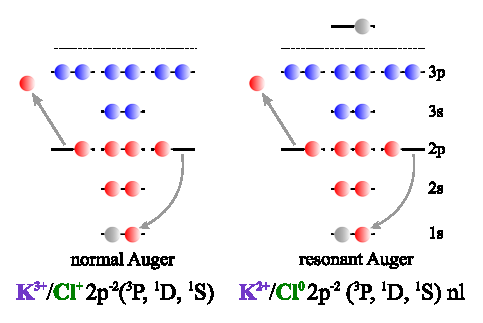
\includegraphics{figures/auger_process.eps}
\caption{Schematic representation of the normal and resonant Auger processes.}
\label{fg:auger}
\end{figure}